% !TEX TS-program = pdflatexmk

\documentclass[14pt]{beamer}
\usepackage{newtxtext,newtxmath}
\usepackage{microtype}
\usepackage[english]{babel}
\usepackage{hyperref}
\usepackage{graphicx}
\usepackage{listings}
\lstloadlanguages{Python}
\lstset{language=Python}
\lstset{%
basicstyle=\ttfamily\bfseries,
keywordstyle=\color{blue}, emph={self}, emphstyle={\color{blue}},
identifierstyle=,
commentstyle=\color{brown},
stringstyle=\color{green!50!black},
showstringspaces=false,
emphstyle={[2]\color{purple}},
}
\usepackage{tikz}
\usepackage{pgfplots}
\usepackage{forest}
\usetikzlibrary{calc}
\usetikzlibrary{shapes}
\usetikzlibrary{positioning}
\usetikzlibrary{arrows}
\usepackage{array}
\newcolumntype{L}[1]{>{\raggedright\let\newline\\\arraybackslash\hspace{0pt}}m{#1}}

\mode<presentation>{
\usetheme{Madrid}
\definecolor{uabgreen}{cmyk}{.89,.31,.78,.17}
\usecolortheme[named=uabgreen]{structure}
\setbeamertemplate{navigation symbols}{}
\setbeamertemplate{footline}[frame number]
\setbeamertemplate{section in toc}[square]
\setbeamertemplate{subsection in toc}[square]
\setbeamertemplate{items}[square]
\setbeamercovered{transparent=5}
}

\newcommand{\keyword}[1]{{\color{blue}#1}}
\newcommand{\cmnt}[1]{{\color{gray}#1}}
\newcommand{\str}[1]{{\color{green!50!black}#1}}
\newcommand{\num}[1]{{\color{green!55!blue}#1}}
\newcommand{\defn}[1]{{\color{purple}#1}}

\newcommand{\limpl}{\Rightarrow}
\newcommand{\liff}{\Leftrightarrow}

\newcommand{\tab}{\hspace{1em}}

\author[Dr. Bethard]{Dr. Steven Bethard}
\institute[UAB CIS]{%
Computer and Information Sciences\\
University of Alabama at Birmingham}

\AtBeginSection[]
{
  \begin{frame}<beamer>{Outline}
    \tableofcontents[currentsection]
  \end{frame}
}

\tikzset{
  invisible/.style={opacity=0,text opacity=0},
  text visible on/.code={%
    \alt<#1>{}{\pgfkeysalso{text opacity=0}}
  },
  visible on/.code={%
    \alt<#1>{}{\pgfkeysalso{invisible}}
  },
  filled on/.code={%
    \alt<#1>{\pgfkeysalso{fill=gray}}{}
  },
  alt/.code n args={3}{%
    \alt<#1>{\pgfkeysalso{#2}}{\pgfkeysalso{#3}}
  },
}
\forestset{
  edge weight/.style={
    edge label={node[midway,above,sloped]{#1}}},
  invisible/.style={
    /tikz/invisible,
    edge={/tikz/invisible}},
  visible on filled on/.code n args={2}{%
    \alt<#1>{\alt<#2>{\pgfkeysalso{fill=gray}}{}}{\pgfkeysalso{invisible}}
  },
  visible on/.code={%
    \alt<#1>{}{\pgfkeysalso{invisible}}
  },
}

\newlength{\wumpusgridsize}
\newenvironment{wumpusgrid}[2]{%
\setlength{\wumpusgridsize}{#2}
\begin{tikzpicture}
\draw[very thick,step=\wumpusgridsize] (0,0) grid (#1\wumpusgridsize, #1\wumpusgridsize);
}{%
\end{tikzpicture}
}
\newcommand{\wumpustop}[5][]{%
\only<#2>{\node[#1] at (#3\wumpusgridsize+0.5\wumpusgridsize,#4\wumpusgridsize+0.75\wumpusgridsize) {#5};}
}
\newcommand{\wumpusbottom}[5][]{%
\only<#2>{\node[#1] at (#3\wumpusgridsize+0.5\wumpusgridsize,#4\wumpusgridsize+0.25\wumpusgridsize) {#5};}
}
\newcommand{\wumpusagent}[3]{\wumpusbottom{#1}{#2}{#3}{\fbox{A}}}
\newcommand{\wumpuspercept}[4]{%
\only<#1>{\node[red,inner sep=0pt] at (#2\wumpusgridsize+0.25\wumpusgridsize,#3\wumpusgridsize+0.75\wumpusgridsize) {\textbf{#4}};}
}
\newcommand{\wumpusknowledge}[4]{%
\only<#1>{\node[draw,cloud,inner sep=0pt,text width=1em,align=center] at (#2\wumpusgridsize+0.75\wumpusgridsize,#3\wumpusgridsize+0.75\wumpusgridsize) {\footnotesize #4};}
}


\pgfplotsset{
    y noise/.style={
        y filter/.code={\pgfmathparse{\pgfmathresult+rnd*#1-0.5*#1}}
    }
}
\forestset{
  decision/.style={draw,fill=gray,minimum height=2em,minimum width=2em,inner sep=0.2em},
  choice/.style={edge label={node[near end,left,inner sep=0.2em]{#1}}},
  result/.style={draw,rounded corners,minimum height=2em,minimum width=2em,inner sep=0.2em},
  decision tree/.style n args={3}{
    for tree={
      s sep=#1,
      l sep=#2,
      align=center,
      edge={thick,-latex},
      % square edges: http://tex.stackexchange.com/questions/108710/square-edges-in-forest-package
      edge path={\noexpand\path[\forestoption{edge}] (\forestOve{\forestove{@parent}}{name}.parent anchor) -- +(0,-#3)-| (\forestove{name}.child anchor)\forestoption{edge label};},
    }
  },
}

\title{Learning from Examples}
\date[]{20 Mar 2014}

\begin{document}

\begin{frame}
  \titlepage
\end{frame}

\begin{frame}{Outline}
  \tableofcontents
\end{frame}

\section{Supervised Learning}

\subsection{Hypothesis Functions}

\begin{frame}{Supervised Learning}
\begin{block}{Key Ideas}
\begin{itemize}
\item Examine pairs of inputs and outputs
\item Guess a possible function mapping input to output
\item Predict outputs given new inputs
\end{itemize}
\end{block}
\bigskip
\begin{columns}
\begin{column}<2->{0.25\textwidth}
$
\begin{array}{lll}
f(1) & = & 1 \\
f(2) & = & 4 \\
f(3) & = & 9 \\
f(4) & = & 16 \\
f(5) & = & \alt<3->{\alert{25}}{?} \\
\end{array}
$
\end{column}
\begin{column}<4->{0.7\textwidth}
\begin{tabular}{lll}
$f$(Romeo and Juliet) & = & Shakespeare \\
$f$(Tom Sawyer)       & = & Twain \\
$f$(Macbeth)          & = & Shakespeare \\
$f$(Huckleberry Finn) & = & Twain \\
$f$(Othello)          & = & \alt<5->{\alert{Shakespeare}}{?} \\
\end{tabular}
\end{column}
\end{columns}
\end{frame}

\begin{frame}{Supervised Learning Components}
\begin{block}{Original Function}
An unknown function $f\!: D_f \rightarrow R_f$
\end{block}
\pause
\begin{block}{Training Examples}
Pairs of $(x, f(x))$ where $x \in D_f$ and $f(x) \in R_f$
\end{block}
\pause
\begin{block}{Hypothesis Function}
Some function $h\!: D_f \rightarrow R_f$
\end{block}
\pause
\begin{block}{Learning Goal}
Pick a hypothesis $h$ as close to $f$ as possible
\end{block}
\end{frame}

\begin{frame}{Problem Formulation}
\begin{block}{Defining a Machine Learning Problem}
Describe the function $f\!: D_f \rightarrow R_f$
\begin{itemize}
\item What is $D_f$?
\item What is $R_f$?
\end{itemize}
\end{block}
\begin{columns}
\begin{column}{0.47\textwidth}<2->
\begin{block}{Ex: Income Prediction}
\begin{description}[$D_f$]
\item[$D_f$] = \uncover<3->{people}
\item[$R_f$] = \uncover<4->{$\mathbb{R}$}
\end{description}
\end{block}
\end{column}
\begin{column}{0.47\textwidth}<5->
\begin{block}{Ex: Face Recognition}
\begin{description}[$D_f$]
\item[$D_f$] = \uncover<6->{images}
\item[$R_f$] = \uncover<7->{image regions}
\end{description}
\end{block}
\end{column}
\end{columns}
\end{frame}

\subsection{Features}

\begin{frame}{Decomposing Domain Objects}
\begin{columns}[T]
\begin{column}{0.4\textwidth}
Smoker identification: \\
\smallskip
\begin{tabular}{lll}
$f$(John)  & = & \textit{true} \\
$f$(Mary)  & = & \textit{false} \\
$f$(Frank) & = & \textit{false} \\
$f$(Sally) & = & ?
\end{tabular}
\end{column}
\pause
\begin{column}{0.55\textwidth}
Easier if we know, e.g.
\begin{itemize}
\item cigarette smell?
\item teeth stains?
\item deep cough?
\end{itemize}
\end{column}
\end{columns}
\bigskip
\pause
\begin{block}{Definition}
\alert{Features} (or \alert{attributes}) are the components of a domain object believed to be important for learning the function $f$
\end{block}
\end{frame}

\begin{frame}{Part of Speech Tagging Example}
\setbeamercovered{invisible}
\begin{tabular}{llllll}
\textcolor{uabgreen}{Input}  & \em John & \em broke & \em the & \em red & \em lamp \\
\textcolor{uabgreen}{Output} & \sc Noun & \sc Verb  & \sc Det & \sc Adj & \sc Noun \\
\end{tabular}
\begin{block}{Function Description}<2->
\begin{description}[$D_f$]
\item[$D_f$] = \uncover<3->{$\{\textit{a},\textit{aardvark},\textit{abacus},\textit{abalone},\ldots\}$ \uncover<6->{\alert<6->{in a sentence}}}
\item[$R_f$] = \uncover<4->{$\{\textsc{Noun},\textsc{Verb},\textsc{Adj},\textsc{Adv},\textsc{Det},\ldots\}$}
\end{description}
\end{block}
\medskip
\begin{columns}<5->
\begin{column}{0.45\textwidth}
$f$(\textit{bark}) = \textsc{Noun}? \textsc{Verb}?
\end{column}
\begin{column}{0.5\textwidth}
\emph{\ldots the \textbf{bark} of the tree \ldots} \\
\emph{\ldots heard the dog \textbf{bark} \ldots} \\
\end{column}
\end{columns}
\begin{block}{Feature Representation}<7->
$\begin{array}{lll}
f([w_{0}\!=\!\textit{bark}, w_{-1}\!=\!\textit{the}]) & = & \textsc{Noun} \\
f([w_{0}\!=\!\textit{bark}, w_{-1}\!=\!\textit{dog}]) & = & \textsc{Verb}
\end{array}$
\end{block}
\end{frame}

\begin{frame}{Named Entity Recognition Exercise}
\begin{block}{Definition}
A \alert{named entity recognition} program find spans of words that are people, locations, organizations, etc.\\
\medskip
\begin{description}[Output]
\item[Input] Bill works for Microsoft Corporation
\item[Output]
$[_{\textsc{\scriptsize Per}}$ Bill$]$ works for
$[_{\textsc{\scriptsize Org}}$ Microsoft Corporation$]$
\end{description}
\end{block}
\begin{block}{Exercise}
Named entity recognition as supervised learning:
\begin{itemize}
\item Describe the function domain
\item Describe the function range
\item Describe the feature space
\end{itemize}
\end{block}
\end{frame}

\begin{frame}{One Named Entity Recognition Approach}
\begin{block}{Function Description}
\begin{description}[$D_f$]
\item[$D_f$] = $\{\textit{a},\textit{aardvark},\textit{abacus},\textit{abalone},\ldots\}$ in a sentence
\item[$R_f$] = $\{\textsc{B-Per},\textsc{I-Per},\textsc{B-Org},\textsc{I-Org},\ldots,\textsc{O}\}$
\end{description}
\end{block}
$\begin{array}{lll}
f(\textit{Bill})        & = & \textsc{B-Per} \\
f(\textit{works})       & = & \textsc{O} \\
f(\textit{for})         & = & \textsc{O} \\
f(\textit{Microsoft})   & = & \textsc{B-Org} \\
f(\textit{Corporation}) & = & \textsc{I-Org} \\
\end{array}$
\begin{block}{Typical Features}
\begin{tabular}{p{0.4\textwidth}p{0.4\textwidth}}
Word itself     & Capitalization \\
Preceding label & First in sentence? \\
\end{tabular}
\end{block}
\end{frame}

\subsection{Evaluating Hypotheses}

\begin{frame}{Evaluating Learning Algorithms}
\begin{enumerate}
\item Train learning algorithm on examples $E_{\textit{\scriptsize train}}$
\item Learning algorithm produces a hypothesis $h$
\item Test hypothesis on new examples $E_{\textit{\scriptsize test}}$ \uncover<2->{- \alert{Don't peek!}}
\end{enumerate}
\begin{columns}
\begin{column}<3->{2in}
Train:
$
\begin{array}[t]{ll|l}
x_1 & x_2 & f(x) \\
\hline
0   & a   & \textit{true} \\
0   & b   & \textit{false} \\
0   & c   & \textit{false} \\
1   & b   & \textit{false} \\
\end{array}
$
\end{column}
\begin{column}<6->{2in}
Test:
$
\begin{array}[t]{ll|l}
x_1 & x_2 & f(x) \\
\hline
1   & a   & \textit{true} \\
0   & b   & \textit{false} \\
0   & c   & \textit{false} \\
1   & c   & \textit{true} \\
\end{array}
$
\end{column}
\end{columns}
\begin{columns}
\begin{column}<4->{2in}
\begin{block}{Algorithm 1}
Always classify as \textit{false}
\\
\uncover<7->{\tab Performance:} \uncover<8->{$\frac{2}{4} = 0.5$}
\end{block}
\end{column}
\begin{column}<5->{2in}
\begin{block}{Algorithm 2}
If $a$ then \textit{true}, else \textit{false}
\\
\uncover<7->{\tab Performance:} \uncover<9->{$\frac{3}{4} = 0.75$}
\end{block}
\end{column}
\end{columns}
\end{frame}

\begin{frame}{Train, Development and Test sets}
\begin{block}{Bad Idea}
\begin{enumerate}
\item\label{item:evaluate} Evaluate on test set
\item Examine errors and adjust hypothesis
\item Goto \ref{item:evaluate}
\end{enumerate}
\end{block}
\pause
\alert{Tuning to your test set} will overestimate model accuracy\\
\pause
\bigskip
Instead, split data into:
\begin{description}[Train]
\item[Train] Used to train a hypothesis function
\item[Dev] Used to tune/adjust the hypothesis
\item[Test] Used to estimate hypothesis function's accuracy
\end{description}
\end{frame}

\begin{frame}[label=cross-validation]{$k$-fold Cross Validation}
Split data into $k$ parts, then iteratively \textcolor{blue!60!white}{train} and \textcolor{uabgreen}{test}:

\begin{tikzpicture}
\fill[alt={10-}{uabgreen}{blue!60!white}](0,0) rectangle (1,1);
\fill[alt={9}{uabgreen}{blue!60!white}](1,0) rectangle (2,1);
\fill[alt={8}{uabgreen}{blue!60!white}](2,0) rectangle (3,1);
\fill[alt={7}{uabgreen}{blue!60!white}](3,0) rectangle (4,1);
\fill[alt={6}{uabgreen}{blue!60!white}](4,0) rectangle (5,1);
\fill[alt={5}{uabgreen}{blue!60!white}](5,0) rectangle (6,1);
\fill[alt={4}{uabgreen}{blue!60!white}](6,0) rectangle (7,1);
\fill[alt={3}{uabgreen}{blue!60!white}](7,0) rectangle (8,1);
\fill[alt={2}{uabgreen}{blue!60!white}](8,0) rectangle (9,1);
\fill[alt={1}{uabgreen}{blue!60!white}](9,0) rectangle (10,1);
\end{tikzpicture}
\uncover<11->{Accuracy is average of the accuracies on each of the $k$ folds}\\
\bigskip
\uncover<12->{
Warnings:
\begin{itemize}
\item Cross validation is \alert{not} a substitution for a test set
\item Cross validation \textcolor{uabgreen}{can be} used instead of train+dev
\end{itemize}
}
\end{frame}


\subsection{Overfitting and Underfitting}

\begin{frame}[label=learning-curves]{Learning Curves}
\begin{center}
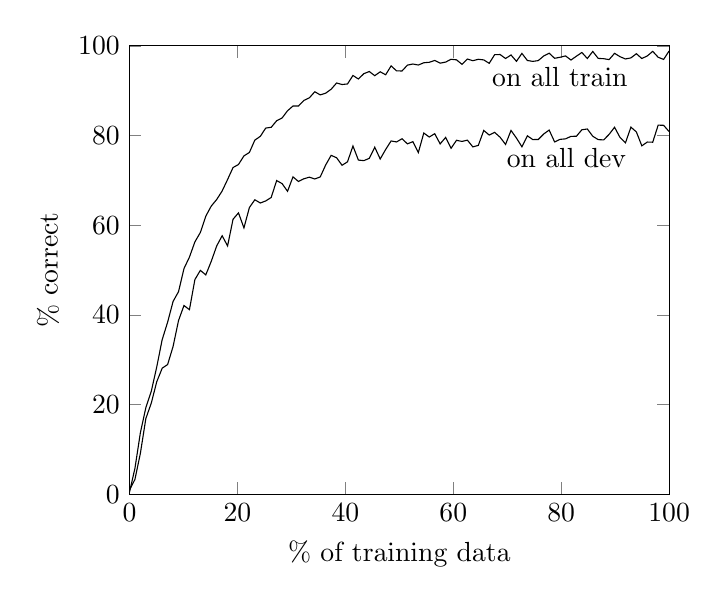
\begin{tikzpicture}
\begin{axis}[
    xmin=0, xmax=100,
    ymin=0, ymax=100,
    xlabel={\% of training data},
    ylabel={\% correct}]
]
\addplot[domain=0:100,samples=100,y noise=2]
plot (\x,{98 - 98*2^(-(\x/10))})
node [pos=0.85,below] {on all train};
\addplot[domain=0:100,samples=100,y noise=5]
plot (\x,{80 - 80*2^(-(\x/10))})
node [pos=0.85,below] {on all dev};
\end{axis}
\end{tikzpicture}
\end{center}
\end{frame}

\begin{frame}[label=insufficient-data]{Insufficient Training Data}
\begin{center}
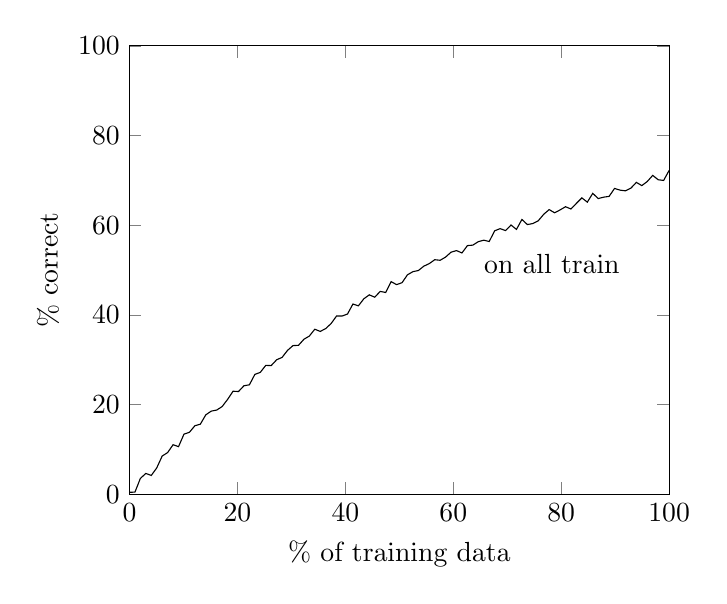
\begin{tikzpicture}
\begin{axis}[
    xmin=0, xmax=100,
    ymin=0, ymax=100,
    xlabel={\% of training data},
    ylabel={\% correct}]
]
\addplot[domain=0:100,samples=100,y noise=2]
plot (\x,{95 - 95*2^(-(\x/50))})
node [pos=0.65,below right] {on all train};
\end{axis}
\end{tikzpicture}
\end{center}
\end{frame}

\begin{frame}[label=underfitting]{Underfitting}
\begin{center}
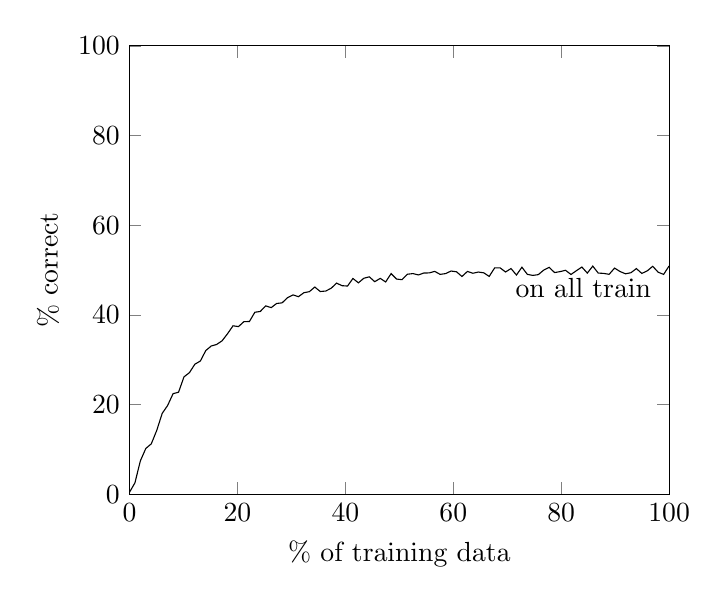
\begin{tikzpicture}
\begin{axis}[
    xmin=0, xmax=100,
    ymin=0, ymax=100,
    xlabel={\% of training data},
    ylabel={\% correct}]
]
\addplot[domain=0:100,samples=100,y noise=2]
plot (\x,{50 - 50*2^(-(\x/10))})
node [pos=0.85,below] {on all train};
\end{axis}
\end{tikzpicture}
\end{center}
\end{frame}

\begin{frame}[label=addressing-underfitting]{Addressing Underfitting}
\small
\begin{columns}
\begin{column}{0.32\textwidth}
\centering
\invisible{Initial}\\
\bigskip
$\begin{array}{ r r | r }
\hline
x_1 & f(x) & h(x) \\
\hline
1 & 1 & 1 \\
2 & 0 & 2 \\
3 & 1 & 3 \\
4 & 4 & 4 \\
\hline
\end{array}$\\
\bigskip
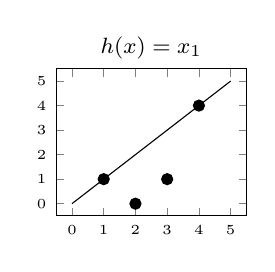
\begin{tikzpicture}
\begin{axis}[
    title={$h(x) = x_1$},
    tiny
]
\addplot[only marks] table[row sep=\\] {
1 1\\
2 0\\
3 1\\
4 4\\
};
\addplot[domain=0:5,samples=10,smooth] plot (\x,\x);
\end{axis}
\end{tikzpicture}
\end{column}
\pause
\begin{column}{0.32\textwidth}
\centering
More complex model\\
\bigskip
$\begin{array}{ r r | r }
\hline
x_1 & f(x) & h(x) \\
\hline
1 & 1 & 1 \\
2 & 0 & 0 \\
3 & 1 & 1 \\
4 & 4 & 4 \\
\hline
\end{array}$\\
\bigskip
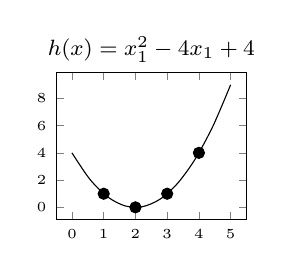
\begin{tikzpicture}
\begin{axis}[
    title={$h(x) = x_1^2 - 4x_1 + 4$},
    tiny
]
\addplot[only marks] table[row sep=\\] {
1 1\\
2 0\\
3 1\\
4 4\\
};
\addplot[domain=0:5,samples=10,smooth] plot (\x,\x^2 - 4*\x + 4);
\end{axis}
\end{tikzpicture}
\end{column}
\pause
\begin{column}{0.32\textwidth}
\centering
More features\\
\bigskip
$\begin{array}{ r r r | r }
\hline
x_1 & x_2 & f(x) & h(x) \\
\hline
1 & 1 & 1 & 1 \\
2 & 4 & 0 & 0 \\
3 & 9 & 1 & 1 \\
4 & 16 & 4 & 4 \\
\hline
\end{array}$\\
\bigskip
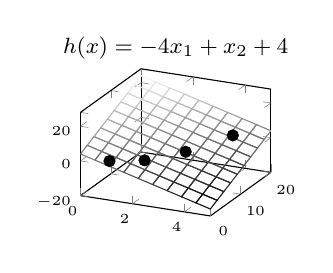
\begin{tikzpicture}
\begin{axis}[
    title={$h(x) = -4x_1 + x_2 + 4$},
    tiny,
    colormap={bw}{gray=(0); gray=(1)},
]
\addplot3[only marks] table[row sep=\\] {
1 1 1\\
2 4 0\\
3 9 1\\
4 16 4\\
};
\addplot3[mesh,domain=0:5,y domain=0:20,samples=10] plot {-4*x + y + 4};
\end{axis}
\end{tikzpicture}
\end{column}
\end{columns}
\end{frame}

\begin{frame}[label=overfitting]{Overfitting}
\begin{center}
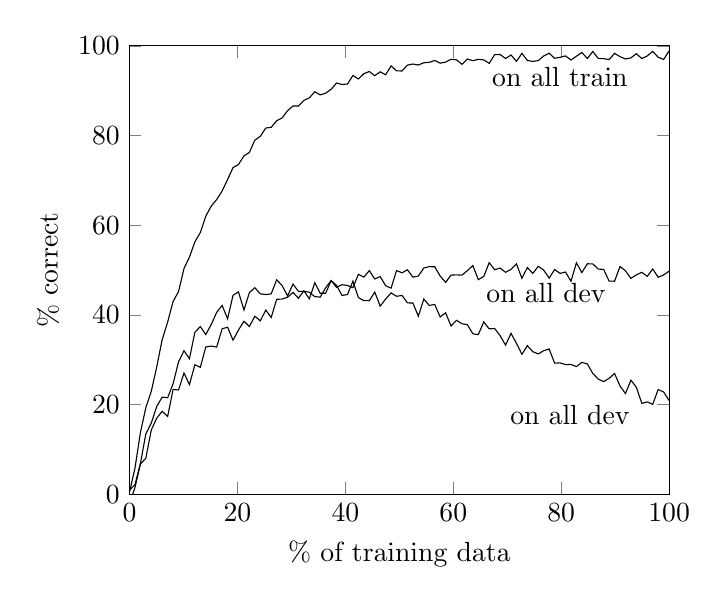
\begin{tikzpicture}
\begin{axis}[
    xmin=0, xmax=100,
    ymin=0, ymax=100,
    xlabel={\% of training data},
    ylabel={\% correct}]
]
\addplot[domain=0:100,samples=100,y noise=2]
plot (\x,{98 - 98*2^(-(\x/10))})
node [pos=0.85,below] {on all train};
\alt<2->{
\addplot[domain=0:100,samples=100,y noise=5]
plot (\x,{70 - 70*2^(-(\x/10)) - x/2})
node [pos=0.95,below left] {on all dev};
}{
\addplot[domain=0:100,samples=100,y noise=5]
plot (\x,{50 - 50*2^(-(\x/10))})
node [pos=0.8,below] {on all dev};
}
\end{axis}
\end{tikzpicture}
\end{center}
\end{frame}

\begin{frame}[label=addressing-overfitting]{Addressing Overfitting}
\small
\begin{columns}[t]
\begin{column}{0.32\textwidth}
\centering
\invisible{Initial}\\
\bigskip
$\begin{array}{ r r r | r }
\hline
x_1 & x_2 & f(x) & h(x) \\
\hline
2 & 1 & 7 & 7\\
3 & 2 & 9 & 9\\
4 & 3 & 13 & 13\\
\hline
\visible<2->{
\color{uabgreen} 1 & \color{uabgreen} 2 & \color{uabgreen} 3 & 1\\
\color{uabgreen} 5 & \color{uabgreen} 1 & \color{uabgreen} 15 & 28\\
\hline
}
\end{array}$\\
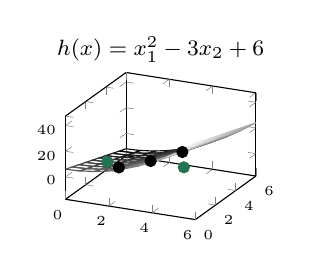
\begin{tikzpicture}
\begin{axis}[
  title={$h(x) = x_1^2-3x_2+6$},
  tiny,
  colormap={bw}{gray=(0); gray=(1)},
]
\addplot3[only marks] table[row sep=\\] {
2 1 7\\
3 2 9\\
4 3 13\\
};
\alt<2->{
\addplot3[only marks,uabgreen] table[row sep=\\] {
1 2 3\\
5 1 15\\
};
}{}
\addplot3[mesh,domain=0:6,samples=10] plot {x^2-3*y+6};
\end{axis}
\end{tikzpicture}
\end{column}
\begin{column}{0.32\textwidth}<3->
\centering
Simpler model\\
\bigskip
$\begin{array}{ r r r | r }
\hline
x_1 & x_2 & f(x) & h(x) \\
\hline
2 & 1 & 7 & 5\\
3 & 2 & 9 & 9\\
4 & 3 & 13 & 13\\
\hline
\color{uabgreen} 1 & \color{uabgreen} 2 & \color{uabgreen} 3 & 3\\
\color{uabgreen} 5 & \color{uabgreen} 1 & \color{uabgreen} 15 & 14\\
\hline
\end{array}$\\
\bigskip
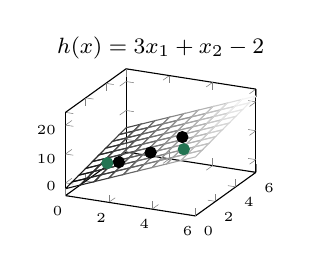
\begin{tikzpicture}
\begin{axis}[
  title={$h(x) = 3x_1+x_2-2$},
  tiny,
  colormap={bw}{gray=(0); gray=(1)},
]
\addplot3[only marks] table[row sep=\\] {
2 1 7\\
3 2 9\\
4 3 13\\
};
\addplot3[only marks,uabgreen] table[row sep=\\] {
1 2 3\\
5 1 15\\
};
\addplot3[mesh,domain=0:6,samples=10] plot {3*x+y-2};
\end{axis}
\end{tikzpicture}
\end{column}
\begin{column}{0.32\textwidth}<4->
\centering
Fewer features\\
\bigskip
$\begin{array}{ r r | r }
\hline
x_1 & f(x) & h(x) \\
\hline
2 & 7 & 6\\
3 & 9 & 9\\
4 & 13 & 12\\
\hline
\color{uabgreen} 1 & \color{uabgreen} 3 & 3\\
\color{uabgreen} 5 & \color{uabgreen} 15 & 15\\
\hline
\end{array}$\\
\bigskip
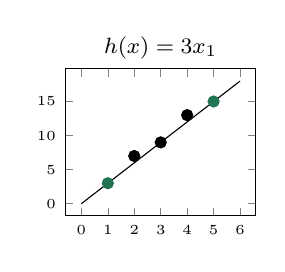
\begin{tikzpicture}
\begin{axis}[
  title={$h(x) = 3x_1$},
  tiny,
  colormap={bw}{gray=(0); gray=(1)},
]
\addplot[only marks] table[row sep=\\] {
2 7\\
3 9\\
4 13\\
};
\addplot[only marks,uabgreen] table[row sep=\\] {
1 3\\
5 15\\
};
\addplot[domain=0:6,samples=10] plot {3*x};
\end{axis}
\end{tikzpicture}
\end{column}
\end{columns}
\end{frame}


\section{Supervised Learning Algorithms}

\subsection{Decision Trees}

\begin{frame}[label=decision-tree-intro]{Decision Trees}
\begin{columns}
\begin{column}{0.6\textwidth}
\centering
Should I play golf today? \\
\bigskip
\small
\begin{forest}
decision tree={1.5em}{3em}{2em}
[{Weather},decision
  [{Humidity},decision,choice={Sunny}
    [{No},result,choice={High}]
    [{Yes},result,choice={Normal}]
  ]
  [{Yes},result,choice={Overcast}]
  [{Wind},decision,choice={Rain}
    [{No},result,choice={Strong}]
    [{Yes},result,choice={Weak}]
  ]
]
\end{forest}
\end{column}
\begin{column}{0.35\textwidth}
\begin{block}{Function}
$D_f$ = days \\
$R_f$ = $\{\textit{Yes}, \textit{No}\}$
\end{block}
\bigskip
\begin{block}{Features}
\begin{itemize}
\item Weather
\item Humidity
\item Wind
\end{itemize}
\end{block}
\end{column}
\end{columns}
\end{frame}

\begin{frame}[label=decision-tree-functions]{Decision Trees as Functions}
\begin{columns}[t]
\begin{column}{0.47\textwidth}
$f(x) = x_1 \textit{ xor } x_2$ \\[1em]
\small
\begin{forest}
decision tree={1.4em}{3em}{2em}
[{$x_1$},decision
  [{$x_2$},decision,choice={true}
    [false,result,choice={true}]
    [true,result,choice={false}]
  ]
  [{$x_2$},decision,choice={false}
    [true,result,choice={true}]
    [false,result,choice={false}]
  ]
]
\end{forest}
\end{column}
\pause
\begin{column}{0.47\textwidth}
$f(x) = (x_1 \land x_2) \lor \lnot x_3$ \\[1em]
\small
\begin{forest}
decision tree={1.4em}{3em}{2em}
[{$x_1$},decision
  [{$x_2$},decision,choice={true}
    [true,result,choice={true}]
    [{$x_3$},decision,choice={false}
      [false,result,choice={true}]
      [true,result,choice={false}]
    ]
  ]
  [{$x_3$},decision,choice={false}
    [false,result,choice={true}]
    [true,result,choice={false}]
  ]
]
\end{forest}
\end{column}
\end{columns}
\end{frame}

\begin{frame}[label=decision-tree-learn]{Learning Decision Trees}
\begin{enumerate}
\item Select a feature $x_i$ for the node
\item For each value of $x_i$ create a child node
\item Sort training examples into child nodes
\item If examples are sorted perfectly, terminate
\item Else, repeat the process for each child node
\end{enumerate}
\begin{columns}
\begin{column}<2->{0.45\textwidth}
$
\begin{array}{cc|c}
x_1          &  x_2          & f(x) \\
\hline
\textit{true}  & \textit{true}   & \textit{true} \\
\textit{true}  & \textit{false}  & \textit{false} \\
\textit{false} & \textit{true}   & \textit{true} \\
\textit{false} & \textit{false}  & \textit{true} \\
\end{array}
$
\end{column}
\begin{column}<3->{0.5\textwidth}
\scriptsize
\begin{forest}
decision tree={1.5em}{3em}{3em}
[{\visible<4->{$x_2$}\\3 true, 1 false},draw,visible on filled on={3-}{4-}
  [{\visible<7->{TRUE}\\\visible<6->{2 true, 0 false}},draw,choice={true},visible on={5-}]
  [{\visible<9->{$x_1$}\\\visible<8->{1 true, 1 false}},draw,choice={false},visible on filled on={5-}{9-}
    [{\visible<12->{FALSE}\\\visible<11->{0 true, 1 false}},draw,choice={true},visible on={10-}]
    [{\visible<14->{TRUE}\\\visible<13->{1 true, 0 false}},draw,choice={false},visible on={10-}]
  ]
]
\end{forest}
\end{column}
\end{columns}
\end{frame}

\begin{frame}[label=decision-tree-exercise]{Decision Tree Exercise}
\setbeamercovered{invisible}
\begin{columns}[t]
\begin{column}{0.4\textwidth}
Build a decision tree for: \\
\bigskip
$
\begin{array}{ll|l}
x_1 & x_2 & f(x) \\
\hline
0   & a   & \textit{true} \\
0   & b   & \textit{false} \\
1   & c   & \textit{true} \\
0   & c   & \textit{false} \\
1   & b   & \textit{false} \\
1   & a   & \textit{true} \\
\end{array}
$
\end{column}
\pause
\begin{column}{0.55\textwidth}
Two possible solutions: \\
\centering
\scriptsize
\bigskip
\begin{forest}
decision tree={1.5em}{2.5em}{1.5em}
[{$x_1$},decision
  [{$x_2$},decision,choice={0}
    [true,result,choice={a}]
    [false,result,choice={b}]
    [false,result,choice={c}]
  ]
  [{$x_2$},decision,choice={1}
    [true,result,choice={a}]
    [false,result,choice={b}]
    [true,result,choice={c}]
  ]
]
\end{forest}\\
\bigskip
\begin{forest}
decision tree={1.5em}{2.5em}{1.5em}
[{$x_2$},decision
  [true,result,choice={a}]
  [false,result,choice={b}]
  [{$x_1$},decision,choice={c}
    [false,result,choice={0}]
    [true,result,choice={1}]
  ]
]
\end{forest}
\end{column}
\end{columns}
\end{frame}

\begin{frame}{Selecting Features for Decision Trees}
\begin{block}{Feature Selection Order}
\begin{itemize}
\item Different orders result in different trees
\item ``Good'' features should be used before ``poor'' ones
\end{itemize}
\end{block}
\pause
\begin{block}{What is a ``good'' feature?}
One whose values predict the class labels \\
\end{block}
\pause
\medskip
\begin{columns}
\begin{column}{1.2in}
$
\begin{array}{lll}
x_1 & x_2 & f(x) \\
\hline
a & 0 & \textit{true} \\
a & 1 & \textit{true} \\
b & 0 & \textit{false} \\
b & 1 & \textit{false} \\
\end{array}
$
\end{column}
\pause
\begin{column}{1.8in}
$x_1$ is a \alert{good} feature \\
\bigskip
$x_2$ is a \alert{poor} feature
\end{column}
\end{columns}
\end{frame}

\begin{frame}{Information}
\begin{block}{Good features provide more information}
Information can be quantified in terms of bits
\end{block}
\pause
Task: Encode \texttt{abacabad} using as few bits as possible
\pause
\medskip
\begin{columns}[t]
\begin{column}{1.8in}
Simple Encoding:
\begin{tabular}{ll}
a & 00 \\
b & 01 \\
c & 10 \\
d & 11 \\
\end{tabular} \\
\pause
\medskip
\texttt{abacabad} $\rightarrow$ 16 bits \texttt{0001001000010011}
\end{column}
\pause
\begin{column}{1.8in}
Using Probability:
\begin{tabular}{ll}
a & 0 \\
b & 10 \\
c & 110 \\
d & 111 \\
\end{tabular} \\
\pause
\medskip
\texttt{abacabad} $\rightarrow$ 14 bits \texttt{01001100100111}
\end{column}
\end{columns}
\pause
\bigskip
\alert{More likely values can be encoded in fewer bits!}
\end{frame}

\begin{frame}{Entropy}
\begin{block}{Definition}
The \alert{entropy} of a random variable $X$ is: \\
\smallskip
\tab\tab$H(X) = -\sum\limits_{x \in X}P(x)\log_2 P(x)$
\end{block}
\pause
\begin{block}{Bit-based Interpretation}
Smallest number of bits that can encode a stream of values from $X$'s distribution
\end{block}
\pause
\begin{block}{Intuitions}
\begin{itemize}
\item High entropy $\rightarrow$ boring (e.g. uniform) distribution
\item Low entropy $\rightarrow$ interesting distribution
\end{itemize}
\end{block}
\end{frame}

\begin{frame}{Entropy}
\begin{columns}
\begin{column}{0.25\textwidth}
\begin{tabular}{ll}
X       & Y   \\
\hline
math    & yes \\
history & no  \\
cs      & yes \\
math    & no  \\
math    & no  \\
cs      & yes \\
history & no  \\
math    & yes \\
\end{tabular}
\end{column}
\begin{column}{0.7\textwidth}
\pause
$
\extrarowheight=2pt
\setlength{\arraycolsep}{0.25em}
\begin{array}{ l l l }
H(X)        & = & \pause -\sum\limits_{x \in X}P(x)\log_2 P(x) \\
     \pause & = & -P(\textit{math})\log_2 P(\textit{math}) \\
            &   & -P(\textit{history})\log_2 P(\textit{history}) \\
            &   & -P(\textit{cs})\log_2 P(\textit{cs}) \\
     \pause & = & -\frac{1}{2}\log_2\frac{1}{2} 
                  -\frac{1}{4}\log_2\frac{1}{4}
                  -\frac{1}{4}\log_2\frac{1}{4} \\
     \pause & = & -\frac{1}{2}(-1) - \frac{1}{4}(-2) - \frac{1}{4}(-2) \\
     \pause & = & \frac{1}{2} + \frac{1}{2} + \frac{1}{2} \\
     \pause & = & 1.5 \\
\\
\pause
H(Y)        & = & \pause 1.0 \\
\end{array}
$
\end{column}
\end{columns}
\end{frame}

\begin{frame}{Specific Conditional Entropy}
\begin{columns}
\begin{column}{0.25\textwidth}
\begin{tabular}{ll}
X               & Y   \\
\hline
math            & yes \\
history         & no  \\
\alert<4-5>{cs} & \alert<4>{yes} \\
math            & no  \\
math            & no  \\
\alert<4-5>{cs} & \alert<4>{yes} \\
history         & no  \\
math            & yes \\
\end{tabular}
\end{column}
\begin{column}{0.7\textwidth}
\begin{block}{Specific Conditional Entropy}
$H(Y|X\!=\!x) = -\sum\limits_{y \in Y}P(y|x)\log_2 P(y|x)$
\end{block}
\small
$
\extrarowheight=2pt
\setlength{\arraycolsep}{0em}
\begin{array}{ l l l }
\uncover<2->{H(Y|X\!=\!\textit{cs})}
& \uncover<2->{=}
& \uncover<3->{\alert<4>{-P(\textit{yes}|\textit{cs})\log_2 P(\textit{yes}|\textit{cs})}}
\\
&
& \uncover<3->{\alert<5>{-P(\textit{no}|\textit{cs})\log_2 P(\textit{no}|\textit{cs})}}
\\
& \uncover<4->{=}
& \uncover<4->{\alert<4>{-1 \log_2 1}}\uncover<5->{\alert<5>{-0 \log_2 0}}
\\
& \uncover<6->{=}
& \uncover<6->{-1 \cdot 0 - 0 \cdot \infty}
\\
& \uncover<7->{=}
& \uncover<7->{0} \\
\end{array}
$ \\
\medskip
\uncover<8->{In other words, $X\!=\!\textit{cs}$ is a great predictor of $Y$}
\end{column}
\end{columns}
\end{frame}

\begin{frame}{Conditional Entropy}
\begin{columns}
\begin{column}{0.25\textwidth}
\begin{tabular}{ll}
X               & Y   \\
\hline
math            & yes \\
history         & no  \\
cs              & yes \\
math            & no  \\
math            & no  \\
cs              & yes \\
history         & no  \\
math            & yes \\
\end{tabular}
\end{column}
\begin{column}{0.7\textwidth}
\setlength{\arraycolsep}{0.25em}
\begin{block}{Conditional Entropy}
$
\begin{array}{ l l l }
H(Y|X) & = & \sum\limits_{x \in X}P(X\!=\!x)H(Y|X\!=\!x)
\end{array}
$
\end{block}
\pause
\small
Given:
$
\begin{array}[t]{ l l l }
H(Y|X\!=\!\textit{math})    & = & 1 \\
H(Y|X\!=\!\textit{history}) & = & 0 \\
H(Y|X\!=\!\textit{cs})      & = & 0 \\
\end{array}
$ \\
\smallskip
\pause
$
\extrarowheight=2pt
\begin{array}{ l l l }
H(Y|X) & = & \pause P(X\!=\!\textit{math}) H(Y|X\!=\!\textit{math}) + \mbox{}\\
       &   & P(X\!=\!\textit{history}) H(Y|X\!=\!\textit{history}) + \mbox{}\\
       &   & P(X\!=\!\textit{cs}) H(Y|X\!=\!\textit{cs}) \\
\pause & = & \frac{1}{2} \cdot 1 + \frac{1}{4} \cdot 0 + \frac{1}{4} \cdot 0 \pause = \frac{1}{2}
\end{array}
$ \\
\medskip
\pause
In other words, $X$ is a good predictor of $Y$
\end{column}
\end{columns}
\end{frame}

\begin{frame}{Information Gain}
\begin{columns}
\begin{column}{0.25\textwidth}
\begin{tabular}{ll}
X               & Y   \\
\hline
math            & yes \\
history         & no  \\
cs              & yes \\
math            & no  \\
math            & no  \\
cs              & yes \\
history         & no  \\
math            & yes \\
\end{tabular}
\end{column}
\begin{column}{0.7\textwidth}
\setlength{\arraycolsep}{0.25em}
\begin{block}{Information Gain}
$IG(Y|X) = H(Y) - H(Y|X)$
\end{block}
\pause
\begin{block}{Intuitive Explanation}
How many bits would it save to know $X$?
\end{block}
\pause
$
\begin{array}[t]{ l l l }
H(Y|X)  & = & 0.5 \\
H(Y)    & = & 1 \\
\\
\pause
IG(Y|X) & = & \pause 1 - 0.5 = 0.5
\end{array}
$
\end{column}
\end{columns}
\end{frame}

\begin{frame}{Decision Trees and Information Gain}
\setbeamercovered{invisible}
Select the feature with the highest information gain:\\
\medskip
\begin{columns}[T]
\begin{column}{0.14\textwidth}
\setlength{\arraycolsep}{0.1em}
\small
$
\begin{array}{ l l l }
X_1 & X_2 & Y \\
\hline
0   & a   & \textsc{t} \\
0   & b   & \textsc{f} \\
1   & c   & \textsc{t} \\
0   & c   & \textsc{f} \\
1   & b   & \textsc{f} \\
1   & a   & \textsc{t} \\
\end{array}
$
\end{column}
\pause
\begin{column}{0.83\textwidth}
\setlength{\arraycolsep}{0.1em}
\small
$
\extrarowheight=2pt
\begin{array}{ l l l l }
H(Y)
& = & \pause -P(\textsc{t})\log_2 P(\textsc{t}) - P(\textsc{f})\log_2 P(\textsc{f}) \\
\pause
& = & -\frac{1}{2}\log_2 \frac{1}{2} - \frac{1}{2}\log_2 \frac{1}{2} \pause = 1 \\
\pause
H(Y|X_1\!\!=\!\!0)
& = & \pause -P(\textsc{t}|0)\log_2 P(\textsc{t}|0) - \pause P(\textsc{f}|0)\log_2 P(\textsc{f}|0) \\
\pause
& = & - \frac{1}{3}\log_2 \frac{1}{3} - \pause \frac{2}{3}\log_2 \frac{2}{3} \pause = 0.92\\
\pause         
H(Y|X_1\!\!=\!\!1)
& = & \pause \ldots = 0.92\\
\pause         
H(Y|X_1)
& = & \pause P(X_1\!\!=\!\!0) H(Y|X_1\!\!=\!\!0) + P(X_1\!\!=\!\!1) H(Y|X_1\!\!=\!\!1) \\
\pause         
& = & 0.5 \cdot 0.92 + \pause 0.5 \cdot 0.92 \pause = 0.92 \\
\pause
IG(Y|X_1)
& = & \pause H(Y) - H(Y|X_1) \pause = 1 - 0.92 \pause = 0.08 \\
\pause         
IG(Y|X_2)
& = & \pause \mbox{\alert{ Your turn! }} \pause = 0.67 \\
\end{array}
$ \\
\medskip
\pause
So $X_2$ is a much better feature to split on
\end{column}
\end{columns}
\end{frame}

\subsection{Random Forests}

\begin{frame}{Random Forests}
\begin{block}{Key Ideas}
\begin{itemize}
\item Voting works better when classifiers are independent
\item Partially random trees should be more independent
\end{itemize}
\end{block}
\pause
\begin{block}{Random Forests}
\begin{enumerate}
\item\label{sample-step} Generate a bootstrap sample of $n$ examples
\item\label{select-step} For each node, select $k$ features at random
\item\label{split-step} Split on the feature with the highest information gain
\item Repeat steps \ref{sample-step}, \ref{select-step} and \ref{split-step} to generate $n$ decision trees
\item Classify by taking the majority vote
\end{enumerate}
\end{block}
\end{frame}

\begin{frame}[label=random-forest-exercise]{Random Forest Example}
\begin{columns}[t]
\begin{column}{0.5\textwidth}
$\begin{array}[t]{lll|l}
x_0 & x_1 & x_2 & f(x) \\
\hline
0   & 0   & 0   & F \\
0   & 0   & 1   & F \\
0   & 1   & 1   & F \\
1   & 0   & 1   & F \\
1   & 0   & 0   & T \\
1   & 1   & 1   & T \\
\end{array}$\\
\bigskip
Bootstrap sample:\\
\tab$[0, 5, 0, 1, 5, 4]$ \\
Random feature subsets:\\
\tab$[1, 2]$, $[2, 0]$
\end{column}
\begin{column}{0.5\textwidth}
\setlength{\arraycolsep}{0em}
\begin{forest}
decision tree={1em}{2.5em}{3em},
for tree={draw,minimum height=3.5em},
baseline
[{{\scriptsize$\begin{array}{ l l l l }
0   & 0   & 0   & F \\
1   & 1   & 1   & T \\
0   & 0   & 0   & F \\
0   & 0   & 1   & F \\
1   & 1   & 1   & T \\
1   & 0   & 0   & T
\end{array}$}
\visible<3->{$x_1$}},visible on filled on={2-}{3-}
  [{{\scriptsize$\begin{array}{ l l l l }
0   & 0   & 0   & F \\
0   & 0   & 0   & F \\
0   & 0   & 1   & F \\
1   & 0   & 0   & T
\end{array}$}
\visible<5->{$x_0$}},choice=0,visible on filled on={4-}{5-}
    [{{\scriptsize$\begin{array}{ l l l l }
0   & 0   & 0   & F \\
0   & 0   & 0   & F \\
0   & 0   & 1   & F \\
\end{array}$}
\visible<7->{$F$}},choice=0,visible on={6-}]
    [{{\scriptsize$\begin{array}{ l l l l }
1   & 0   & 0   & T
\end{array}$}
\visible<7->{$T$}},choice=1,visible on={6-}]
  ]
  [{{\scriptsize$\begin{array}{ l l l l }
1   & 1   & 1   & T \\
1   & 1   & 1   & T \\
\end{array}$}
\visible<7->{$T$}},choice=1,visible on={4-}]
]
\end{forest}
\end{column}
\end{columns}
\end{frame}

\begin{frame}{Random Forest Properties}
\begin{block}{Disadvantages}
\begin{itemize}
\item Hard to estimate complexity due to random factor
\item $k$ (\# of features) must be determined experimentally
\end{itemize}
\end{block}
\pause
\begin{block}{Advantages}
\begin{itemize}
\item State of the art performance on many datasets
\item Relatively simple to implement
\item Expected error can be determined while training
\pause
\begin{itemize}
\item Bootstrap sample leaves out about $\frac{1}{3}$ of examples
\item Use these out-of-bag examples to test individual trees
\item Collect votes from all trees to get overall accuracy
\end{itemize}
\end{itemize}
\end{block}
\end{frame}

\subsection{Linear and Logistic Regression}

\begin{frame}[label=linear-models]{Linear Models}{}
{\Large$h_{\theta}(x) = \theta_0 + \theta_1 x_1 + \theta_2 x_2 + \ldots$}\\[1em]
Where:
\begin{itemize}
\item $x_1, x_2, x_3, \ldots$ are the features of $x$
\item $\theta$ are feature weights
\end{itemize}
\pause
\bigskip
Learning linear models:
\begin{itemize}
\item Select parameters (weights) to minimize \emph{loss}
\end{itemize}
\end{frame}

\begin{frame}[label=loss]{Loss}
\setbeamercovered{invisible}
\begin{columns}
\begin{column}{0.48\textwidth}
How ``wrong'' is this $h(x)$?\\[1em]
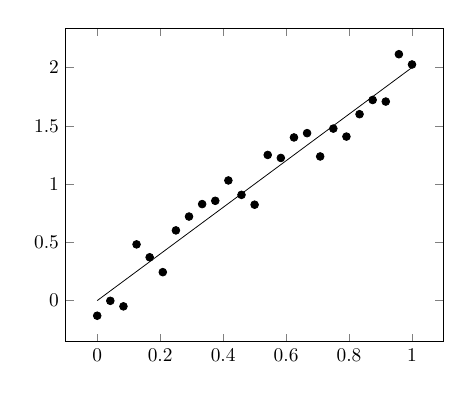
\begin{tikzpicture}[scale=0.7]
\begin{axis}[domain=0:1]
\pgfmathsetseed{42}
\addplot[y noise=0.5, only marks] {2*x};
\addplot[no marks] {2*x};
\end{axis}
\end{tikzpicture}
\end{column}
\pause
\begin{column}{0.48\textwidth}
\setlength{\arraycolsep}{0.1em}
\renewcommand{\arraystretch}{1.75}
\begin{block}{Loss at one point}
$\begin{array}{ l l l }
L_{0/1} & = &
\begin{cases}
0 & \text{if } h(x) = f(x) \\
1 & \text{otherwise}
\end{cases}
\\
\pause L_1 & = & \left| f(x) - h(x) \right| \\
\pause L_2 & = & \left( f(x) - h(x) \right)^2
\end{array}$
\end{block}
\pause
\begin{block}{Empirical Loss}
$\displaystyle\frac{1}{|X|} \sum_{x \in X} L(f(x), h(x))$
\end{block}
\end{column}
\end{columns}
\end{frame}

\begin{frame}[label=loss-exercise]{Loss Exercise}
\begin{columns}
\begin{column}{0.55\textwidth}
Which linear model parameters:
\begin{enumerate}
\item $\theta_1 = [0, 1]$
% L_{0/1} => 2
% L_1 => 6
% L_2 => 20
\item $\theta_2 = [0.6, 1.2]$
% L_{0/1} => 5
% L_1 => 7.2
% L_2 => 12.4
\end{enumerate}
are better by:
\begin{itemize}
\item $L_{0/1}$ loss?
\only<2->{\\ \tab $\theta_1$ (2 vs. 5)}
\item $L_1$ loss?
\only<2->{\\ \tab $\theta_1$ (6 vs. 7.2)}
\item $L_2$ loss?
\only<2->{\\ \tab $\theta_2$ (20 vs. 12.4)}
\end{itemize}
\end{column}
\begin{column}{0.4\textwidth}
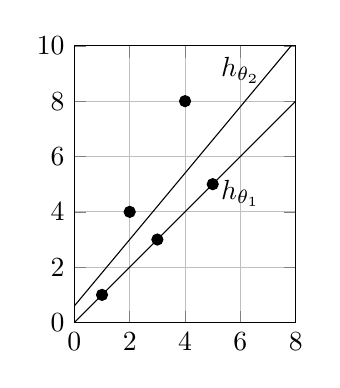
\begin{tikzpicture}
\begin{axis}[
  grid=both,
  xmin=0,ymin=0,
  xmax=8,ymax=10,
  x=1em,y=1em,
  domain=0:8,
]
\pgfmathsetseed{42}
\addplot[only marks] table[row sep=\\] {
1 1\\
2 4\\
3 3\\
4 8\\
5 5\\
};
\only<2->{
\addplot[no marks] {x} node[below=0.5em,near end] {$h_{\theta_1}$};
\addplot[no marks] {0.6 + 1.2*x} node[above=0.5em,near end] {$h_{\theta_2}$};
}
\end{axis}
\end{tikzpicture}
\end{column}
\end{columns}
\end{frame}

\begin{frame}[label=learning-via-loss]{Learning Parameters via Minimizing Loss}
\setbeamercovered{invisible}
\begin{block}{Key Ideas}
\begin{itemize}
\item Best model parameters $\theta = \displaystyle\argmin_{\theta'} Loss(h_{\theta'})$
\item Minimized function has partial derivatives = 0
\end{itemize}
\end{block}
\pause
Example: $x = [x_1]$ with $L_2$ loss\\
\footnotesize\setlength{\arraycolsep}{0.25em}
$\begin{array}{ >{\displaystyle}r >{\displaystyle}c >{\displaystyle}l }
Loss(h_{\theta})
& = & \frac{1}{|X|}\sum_{x \in X} \left(f(x) - (\theta_0 + \theta_1 x_1)\right)^2\\
\pause
& = & \frac{1}{|X|}\sum_{x \in X} f(x)^2 - 2 \theta_0 f(x) - 2 \theta_1 x_1 f(x) + \theta_0^2 + 2 \theta_0 \theta_1 x_1 + \theta_1^2 x_1^2 \\
\pause
\displaystyle\frac{\delta}{\delta\theta_0} Loss(h_{\theta})
& = & \frac{1}{|X|}\sum_{x \in X} - 2 f(x) + 2 \theta_0 + 2 \theta_1 x_1 = 0\\
\pause
\theta_0
& = & \frac{1}{|X|}\sum_{x \in X} f(x) - \theta_1 x_1 \\
\pause
\displaystyle\frac{\delta}{\delta\theta_1} Loss(h_{\theta}) & = & \ldots \\
\end{array}$
\end{frame}

\begin{frame}[label=gradient-descent]{Learning Parameters via Minimizing Loss}
Formal approach:
\begin{itemize}
\item Given: function $h_{\theta}$ and function $Loss(\theta)$
\item Derive $\nabla Loss(\theta) = [\frac{\delta}{\delta\theta_0} Loss(\theta), \frac{\delta}{\delta\theta_1} Loss(\theta), \ldots]$
\item Solve for $\theta$ in $\nabla Loss(\theta) = 0$
\end{itemize}
\pause
But there may be no closed form solution!
\pause
\begin{block}{Gradient Descent}
\tt
$\theta$ = any setting of all parameters\\
\keyword{while} $\theta$ has not converged:\\
\tab \keyword{for} i \keyword{in} $0 \ldots |\theta|$:\\
\tab \tab $\displaystyle \theta_i = \theta_i - \alpha \frac{\delta}{\delta\theta_i} Loss(\theta)$
\end{block}
\end{frame}

\begin{frame}[label=gradient-descent-properties]{Gradient Descent Properties}
For convex functions:
\begin{itemize}
\item Given small enough $\alpha$, converges to global minimum
\item May be slow: scans entire training data every step
\end{itemize}
\pause
\bigskip
Alternative: stochastic gradient descent:
\begin{itemize}
\item Calculate loss for each $x$ and update $\theta$ accordingly
\item Often faster than batch gradient descent
\item Not guaranteed to converge to global minimum
\end{itemize}
\pause
\bigskip
For non-convex functions:
\begin{itemize}
\item Only converges to a local minimum
\end{itemize}
\end{frame}

\begin{frame}[label=regularization]{Avoiding Overfitting with Regularization}
Recall overfitting solutions:
\pause
\begin{itemize}
\item Use simpler model
\item Use fewer features
\end{itemize}
\pause
Learning as optimization allows another: \emph{Regularization}
\begin{itemize}
\item Instead of minimizing $Loss(\theta)$
\item Minimize $Loss(\theta) + \lambda \: Complexity(\theta)$
\item Where $\lambda$ can be tuned
\end{itemize}
\pause
Common choices for $Complexity(\theta)$
\begin{itemize}
\item $\displaystyle L_1(\theta) = \sum_{i} | \theta_{i} |$, encourages weights of 0 (sparsity)
\item $\displaystyle L_2(\theta) = \sum_{i} | \theta_{i} |^{2}$, often makes math easier
\end{itemize}
\end{frame}

\begin{frame}[label=regularization-exercise]{Regularization Exercise}
\begin{columns}
\begin{column}{0.4\textwidth}
Which parameters:
\begin{enumerate}
\item $\theta_1 = [-2, 3, 1]$
% -2 + 6 + 1 = 5
% -2 + 9 + 2 = 9
% -2 + 12 + 3 = 13
% L_2 loss => [1, 0, 0] => 1
% L_1 reg => 2 + 3 + 1 => 6
% L_2 reg => 4 + 9 + 1 => 14
\item $\theta_2 = [0, 3, 0]$
% 6
% 9
% 12
% L_2 loss => [2, 0, 1] => 5
% L_1 reg => 3
% L_2 reg => 9
\end{enumerate}
are better with $L_2$ loss and the regularization:
\begin{itemize}
\item None?
\only<2->{\\ \tab $\theta_1$ (1 vs. 5)}
\item $L_1$ with $\lambda=1$?
\only<2->{\\ \tab $\theta_1$ (7 vs. 8)}
\item $L_2$ with $\lambda=1$?
\only<2->{\\ \tab $\theta_2$ (15 vs. 14)}
\end{itemize}
\end{column}
\begin{column}{0.55\textwidth}
\centering
$\begin{array}{ r r r }
\hline
x_1 & x_2 & f(x) \\
\hline
2 & 1 & 4 \\
3 & 2 & 9 \\
4 & 3 & 13 \\
\hline
\end{array}$\\
\bigskip
\visible<3->{
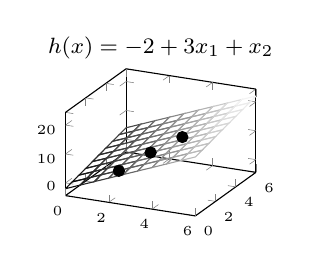
\begin{tikzpicture}
\begin{axis}[
  title={$h(x) = -2 + 3x_1 + x_2$},
  tiny,
  colormap={bw}{gray=(0); gray=(1)},
]
\addplot3[only marks] table[row sep=\\] {
2 1 4\\
3 2 9\\
4 3 13\\
};
\addplot3[mesh,domain=0:6,samples=10] plot {3*x+y-2};
\end{axis}
\end{tikzpicture}
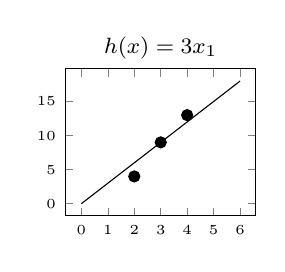
\begin{tikzpicture}
\begin{axis}[
  title={$h(x) = 3x_1$},
  tiny,
  colormap={bw}{gray=(0); gray=(1)},
]
\addplot[only marks] table[row sep=\\] {
2 4\\
3 9\\
4 13\\
};
\addplot[domain=0:6,samples=10] plot {3*x};
\end{axis}
\end{tikzpicture}
}
\end{column}
\end{columns}
\end{frame}

\begin{frame}[label=logistic-regression-intro]{Linear vs. Logistic Regression}
\centering
Linear regression is bad for classification:\\
\bigskip
\begin{tikzpicture}
\begin{axis}[
  domain=-1:7,
  xmin=-0.5,xmax=6.5,ymin=-0.5,ymax=1.5,
  ytick={0,1},
  x=3em,y=5em,
]
\addplot[only marks] table[row sep=\\] {
1 0\\
2 0\\
3 0\\
4 1\\
5 1\\
};
\only<2->{
\addplot[samples=100] plot {0.3 * x - 0.5}
node[midway,left] {\small $h(x) = - 0.5 + 0.3 x$};
}
\only<4->{
\addplot[samples=100,smooth] plot {1 / (1 + e^(-(-140 + 40 * x))) }
node[midway,right] {\small $\displaystyle h(x) = \frac{1}{1 - e^{-(-140 + 40 x)}}$};
}
\end{axis}
\end{tikzpicture}\\
\uncover<3->{
Instead, use \emph{logistic regression}
}
\end{frame}

\begin{frame}[label=logistic-regression]{Linear vs. Logistic Regression}
Linear regression:
\begin{itemize}
\item $h(x): \mathbb{R}^n \Rightarrow \mathbb{R}$
\item $h_{\theta}(x) = \theta_0 + \theta_1 x_1 + \theta_2 x_2 + \ldots$
\item $\displaystyle L_2(h_{\theta}) = \frac{1}{|X|}\sum_{x \in X} \left(f(x) - \left( \theta_0 + \theta_1 x_1 + \theta_2 x_2 + \ldots \right)\right)^2$
\end{itemize}
\pause
Logistic regression:
\begin{itemize}
\item $h(x): \mathbb{R}^n \Rightarrow [0,1]$
\item $\displaystyle h_{\theta}(x) = \frac{1}{1 + e^{-(\theta_0 + \theta_1 x_1 + \theta_2 x_2 + \ldots)}}$
\item $\displaystyle L_2(h_{\theta}) = \frac{1}{|X|}\sum_{x \in X} \left(f(x) - \left( \frac{1}{1 + e^{-(\theta_0 + \theta_1 x_1 + \theta_2 x_2 + \ldots)}} \right)\right)^2$
\end{itemize}
\end{frame}

\begin{frame}[label=logistic-regression-properties]{Logistic Regression Properties}
\begin{itemize}
\item $h_{\theta}(x)$ can be interpreted as $P(f(x) = 1)$
\item Can be generalized for multi-class classification
\item With regularization, state-of-the-art on many problems
\end{itemize}
\end{frame}

\subsection{Support Vector Machines}

\begin{frame}[label=max-margin]{Max Margin Classification}{}
\begin{columns}[t]
\begin{column}{0.47\textwidth}
\centering
Classification problem:\\
\medskip
\only<1>{
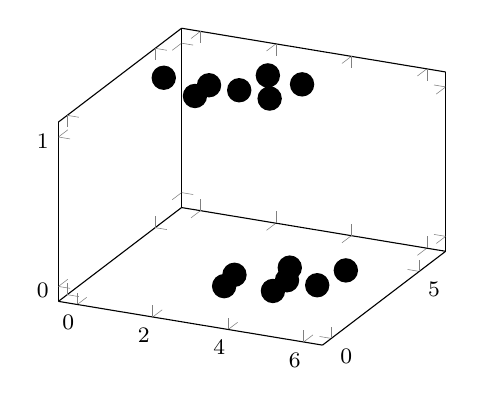
\begin{tikzpicture}
\begin{axis}[
  small,
  colormap/blackwhite,
  ztick={0,1},
  xmin=-0.5,xmax=6.5,
  ymin=-0.5,ymax=6.5,
  domain=-1:7
]
\addplot3[
  only marks,
  mark options={scale=2,thick},
] table[row sep=\\] {
0.1 4.2 1\\
1.3 3.4 1\\
1.3 4.2 1\\
2.1 4.2 1\\
2.3 5.4 1\\
3 4 1\\ % support vector
3.3 5.2 1\\
3.1 1.2 0\\
3 2 0\\ % support vector
4.3 1.4 0\\
4.3 2.2 0\\
4 3 0\\ % support vector
5.1 2.2 0\\
5.3 3.4 0\\
};
\end{axis}
\end{tikzpicture}
}
\only<2->{
\begin{tikzpicture}
\begin{axis}[
  colormap/blackwhite,
  x=1.5em,
  y=1.5em,
  xmin=-0.5,xmax=6.5,
  ymin=-0.5,ymax=6.5,
  domain=-1:7
]
\addplot[
  only marks,
  mark options={scale=2,thick},
] table[row sep=\\] {
0.1 4.2 1\\
1.3 3.4 1\\
1.3 4.2 1\\
2.1 4.2 1\\
2.3 5.4 1\\
3 4 1\\ % support vector
3.3 5.2 1\\
};
\addplot[
  only marks,
  mark options={scale=2,thick,fill=white},
] table[row sep=\\] {
3.1 1.2 0\\
3 2 0\\ % support vector
4.3 1.4 0\\
4.3 2.2 0\\
4 3 0\\ % support vector
5.1 2.2 0\\
5.3 3.4 0\\
};
\only<4-5>{
\addplot[no marks] plot {3.7};
}
\only<6-7,11>{
\addplot[no marks] plot {2 * x - 3};
\only<11>{
\addplot[no marks,domain=3:3.4] plot {-0.5 * x + 5.5};
\addplot[no marks,domain=2.6:3] plot {-0.5 * x + 3.5};
}
}
\only<8-9,12>{
\addplot[no marks] plot {x};
\only<12>{
\addplot[no marks,domain=3:4] plot {-x + 7};
\addplot[no marks,domain=2.5:3] plot {-x + 5};
}
}
\end{axis}
\end{tikzpicture}
}
\end{column}
\begin{column}<3->{0.47\textwidth}
Classification hyperplanes:
\begin{itemize}
\item<4-> $x_2 = 3.7$ \hfill \uncover<5->{$\Rightarrow \frac{13}{14}}$
\item<6-> $2 x_1 - x_2 = 3$ \hfill \uncover<7->{$\Rightarrow \frac{14}{14}}$
\item<8-> $x_1 - x_2 = 0$ \hfill \uncover<9->{$\Rightarrow \frac{14}{14}}$
\end{itemize}
\bigskip
\uncover<10->{
Maximizing margin:
\begin{itemize}
\item<11-> $2 x_1 - x_2 = 3$ \hfill $\Rightarrow 0.35$
\item<12-> $x_1 - x_2 = 0$ \hfill $\Rightarrow 0.50$
\end{itemize}
}
\bigskip
\uncover<13->{
Data points at margin are called \emph{support vectors}
}
\end{column}
\end{columns}
\end{frame}

\begin{frame}[label=svm]{Support Vector Machine Classifiers}
Support vector machine loss, with $f(x): \mathbb{R} \Rightarrow \{-1,+1\}$:\\
$\displaystyle L_2(\theta) =
\underbrace{\frac{1}{2} \sum_{i} \theta_i^{2}}_{\text{regularizer}}
+ \underbrace{C}_{\substack{\text{misclassify}\\\text{cost}}}
\sum_{x \in X}
\max \left( 0,  1 - f(x) \underbrace{\sum_{i} \theta_{i} x_{i}}_{\text{linear model}} \right) $\\
\pause
\bigskip
Compare to L2-regularized logistic regression:\\
$\displaystyle L_2(\theta) =
\frac{1}{2} \sum_{i} \theta_i^{2}
+ \hspace{1em} \frac{1}{|X|} \hspace{1em}
\sum_{x \in X}
\left(f(x) - \left( \frac{1}{1 + e^{-\sum_{i} \theta_{i} x_{i} }} \right)\right)^2$
\end{frame}

\begin{frame}[label=kernels]{Kernel Methods}
Support vector machine dual form:\\
\medskip
$\displaystyle L(\alpha)
= \sum_{x \in X} \alpha_{x}
- \frac{1}{2}\sum_{x \in X, \: x' \in X} \alpha_{x} \alpha_{x'} f(x) f(x')
\alt<2->{k(x, x')}{\sum_{i} x_i x'_i}$\\
\bigskip
\uncover<3->{
Common kernels $k(x,x')$:
\begin{itemize}
\item Linear -- $(\sum_{i} x_i x'_i)$
\item Polynomial -- $(\sum_{i} x_i x'_i)^d$
\item Radial basis function (RBF) -- $\displaystyle e^{-\gamma \| x - x' \|^2}$
\end{itemize}
}
\bigskip
\uncover<4->{
Demo: kernels allow non-linear classification boundaries
\begin{itemize}
\item \small\url{http://www.csie.ntu.edu.tw/~cjlin/libsvm/\#GUI}
\end{itemize}
}
\end{frame}

\begin{frame}[label=kernel-alternative]{Kernel Alternative: Feature Engineering}
Nonlinear classification via feature transformation:
\bigskip
\begin{columns}
\begin{column}{0.45\textwidth}
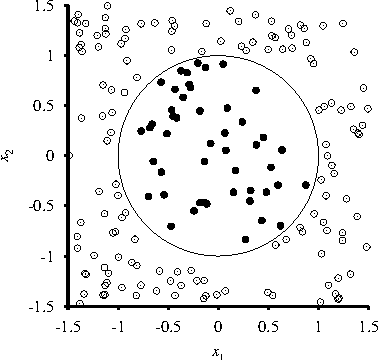
\includegraphics[width=\textwidth]{circle-x1-x2}
\end{column}
\begin{column}{0.45\textwidth}
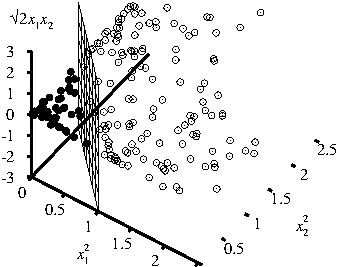
\includegraphics[width=\textwidth]{circle-x1-x2-x1x2}
\end{column}
\end{columns}
\bigskip
\pause
Kernels: similar effect, but may be more efficient
\end{frame}

\begin{frame}[label=svm-properties]{Support Vector Machine Properties}
\begin{block}{Theoretical Properties}
\begin{itemize}
\item Efficient optimal separators in huge feature spaces
\item Can approximate essentially any function
\end{itemize}
\end{block}
\begin{block}{Empirical Issues}
\begin{itemize}
\item Classification usually fast, but training often slow
\item Kernel functions (and parameters) chosen empirically
\end{itemize}
\end{block}
\end{frame}


\part{Key Ideas}

\begin{frame}{Key Ideas}
\begin{block}{Supervised Learning}
\begin{itemize}
\item Input: $(x, f(x))$ examples
\item Output: $h$, a guess at $f$
\item Representation: $x$ decomposed into features
\item Evaluation: train, development, test
\item Learning curves: reveal underfitting, overfitting
\end{itemize}
\end{block}
\begin{block}{Supervised Learning Algorithms}
\begin{itemize}
\item Decision trees via information gain
\item Random forests
\item Linear and logistic regression
\item Support vector machines
\end{itemize}
\end{block}
\end{frame}

\end{document}


